\chapter{Grundlagen des Systems}
\section{Fe(100), Fe(100)-p(1\,x\,1)O und MgO}

Eisen ist bei Raumtemperatur ferromagnetisch und kristalliert in einer kubisch-raumzentrierten Kristallstruktur 
mit einer Gitterkonstante von $2,87\,\si{\angstrom}$. 
Die Bezeichnung Fe(100) bezieht sich auf die Miller-Indizes ($h\,k\,l$) und gibt die Orientierung der Kristalloberfläche im Raum an.

Bei der Passivierung mit Sauerstoff setzen sich die Sauerstoffionen auf die Muldenplätze der Fe(100)-Struktur und bilden eine (1\,x\,1)-Überstruktur \cite{jona1987re}.
Die chemische Stabilität der Oberfläche erhöht sich auf diese Weise und die magnetischen Eigenschaften werden gleichzeitig verstärkt \cite{tange2010electronic}.

\begin{SCfigure}
    \centering
    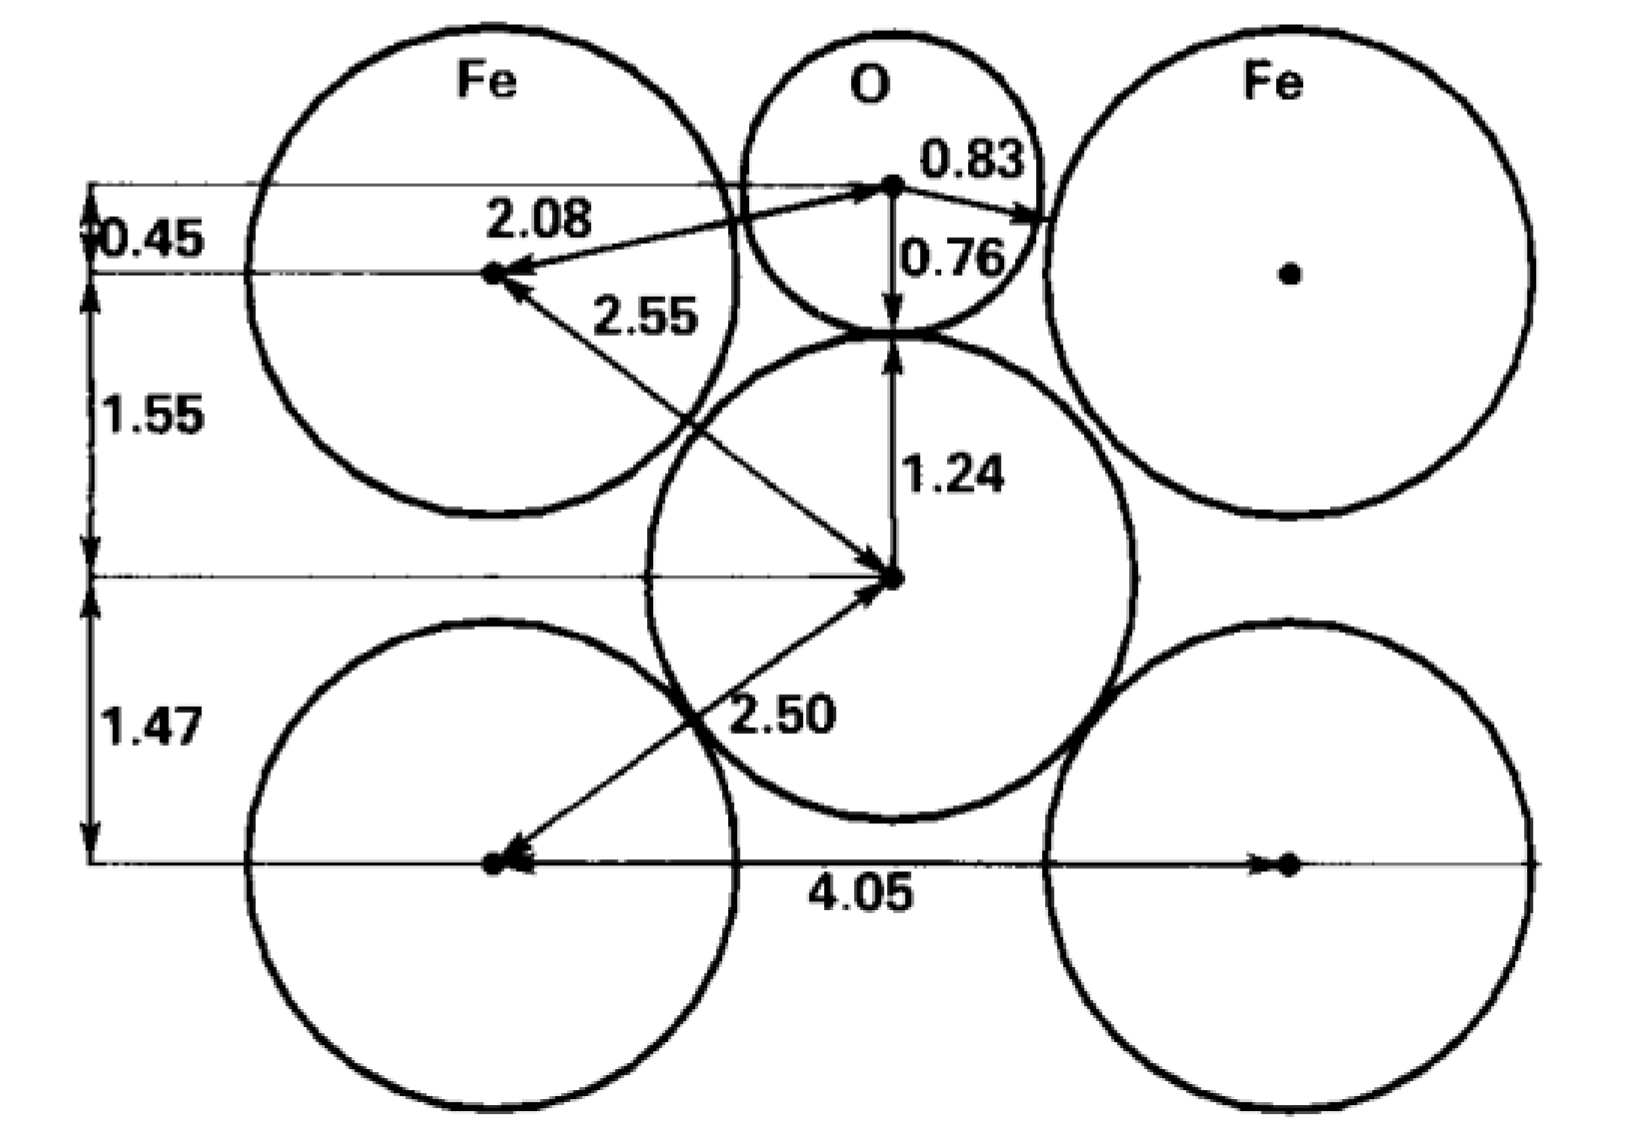
\includegraphics[width=0.45\linewidth]{Plots/FeO_Struktur.png}
    \caption{Schematische Darstellung der Fe(100)-p(1\,x\,1)O-Oberfläche in der Seitenansicht mit Angabe der durch die Passivierung verursachten Deformationen der Fe(100) Oberfläche \cite{jona1987re}.}
    \label{fig:FeO}
\end{SCfigure}

Magnesiumoxid kristallisiert in einer NaCl-Struktur mit einer Gitterkonstante von $4,21\,\si{\angstrom}$.
Eine einzelne Monolage im Festkörper ist demnach $2,105\,\si{\angstrom}$ groß, mit vernachlässigbaren Abweichungen
an der Grenzfläche zu Fe(100)- und Fe(100)-p(1\,x\,1)O-Oberflächen \cite{meyerheim2001geometrical}.




\section{Arten des Schichtwachstums}
\label{sec:Wachstum}

Idealerweise verläuft das Wachstum des Adsorbats lagenweise auf dem Substrat (Frank-van-der-Merwe-Wachstum), sodass Atome erst dann 
eine neue Monolage ("ML") bilden, wenn die vorherige ML vollständig belegt ist.
Ist die Grenzflächenenergie des wachsenden Films zum Substrat und zum Vakuum größer als 
die Energie des Substrats zum Vakuum, so kommt es zu Inselwachstum (Volmer-Weber-Wachstum).
Da es energetisch günstiger ist, möglichst wenig Fläche des Substrats zu bedecken, bildet sich ein Film, der weder einkristallin 
noch von homogener Dicke ist.
Wird dem System Energie in Form von Wärme zugefügt, kann diese Energiedifferenz überwunden werden und bevorzugt ein lagenweises Wachstum 
stattfinden. Die Mischform aus anfänglich lagenweisem Wachstum und anschließendem Inselwachstum wird Stranski-Krastanov-Wachstum genannt \cite{fauster}.

\begin{SCfigure}
    \centering
    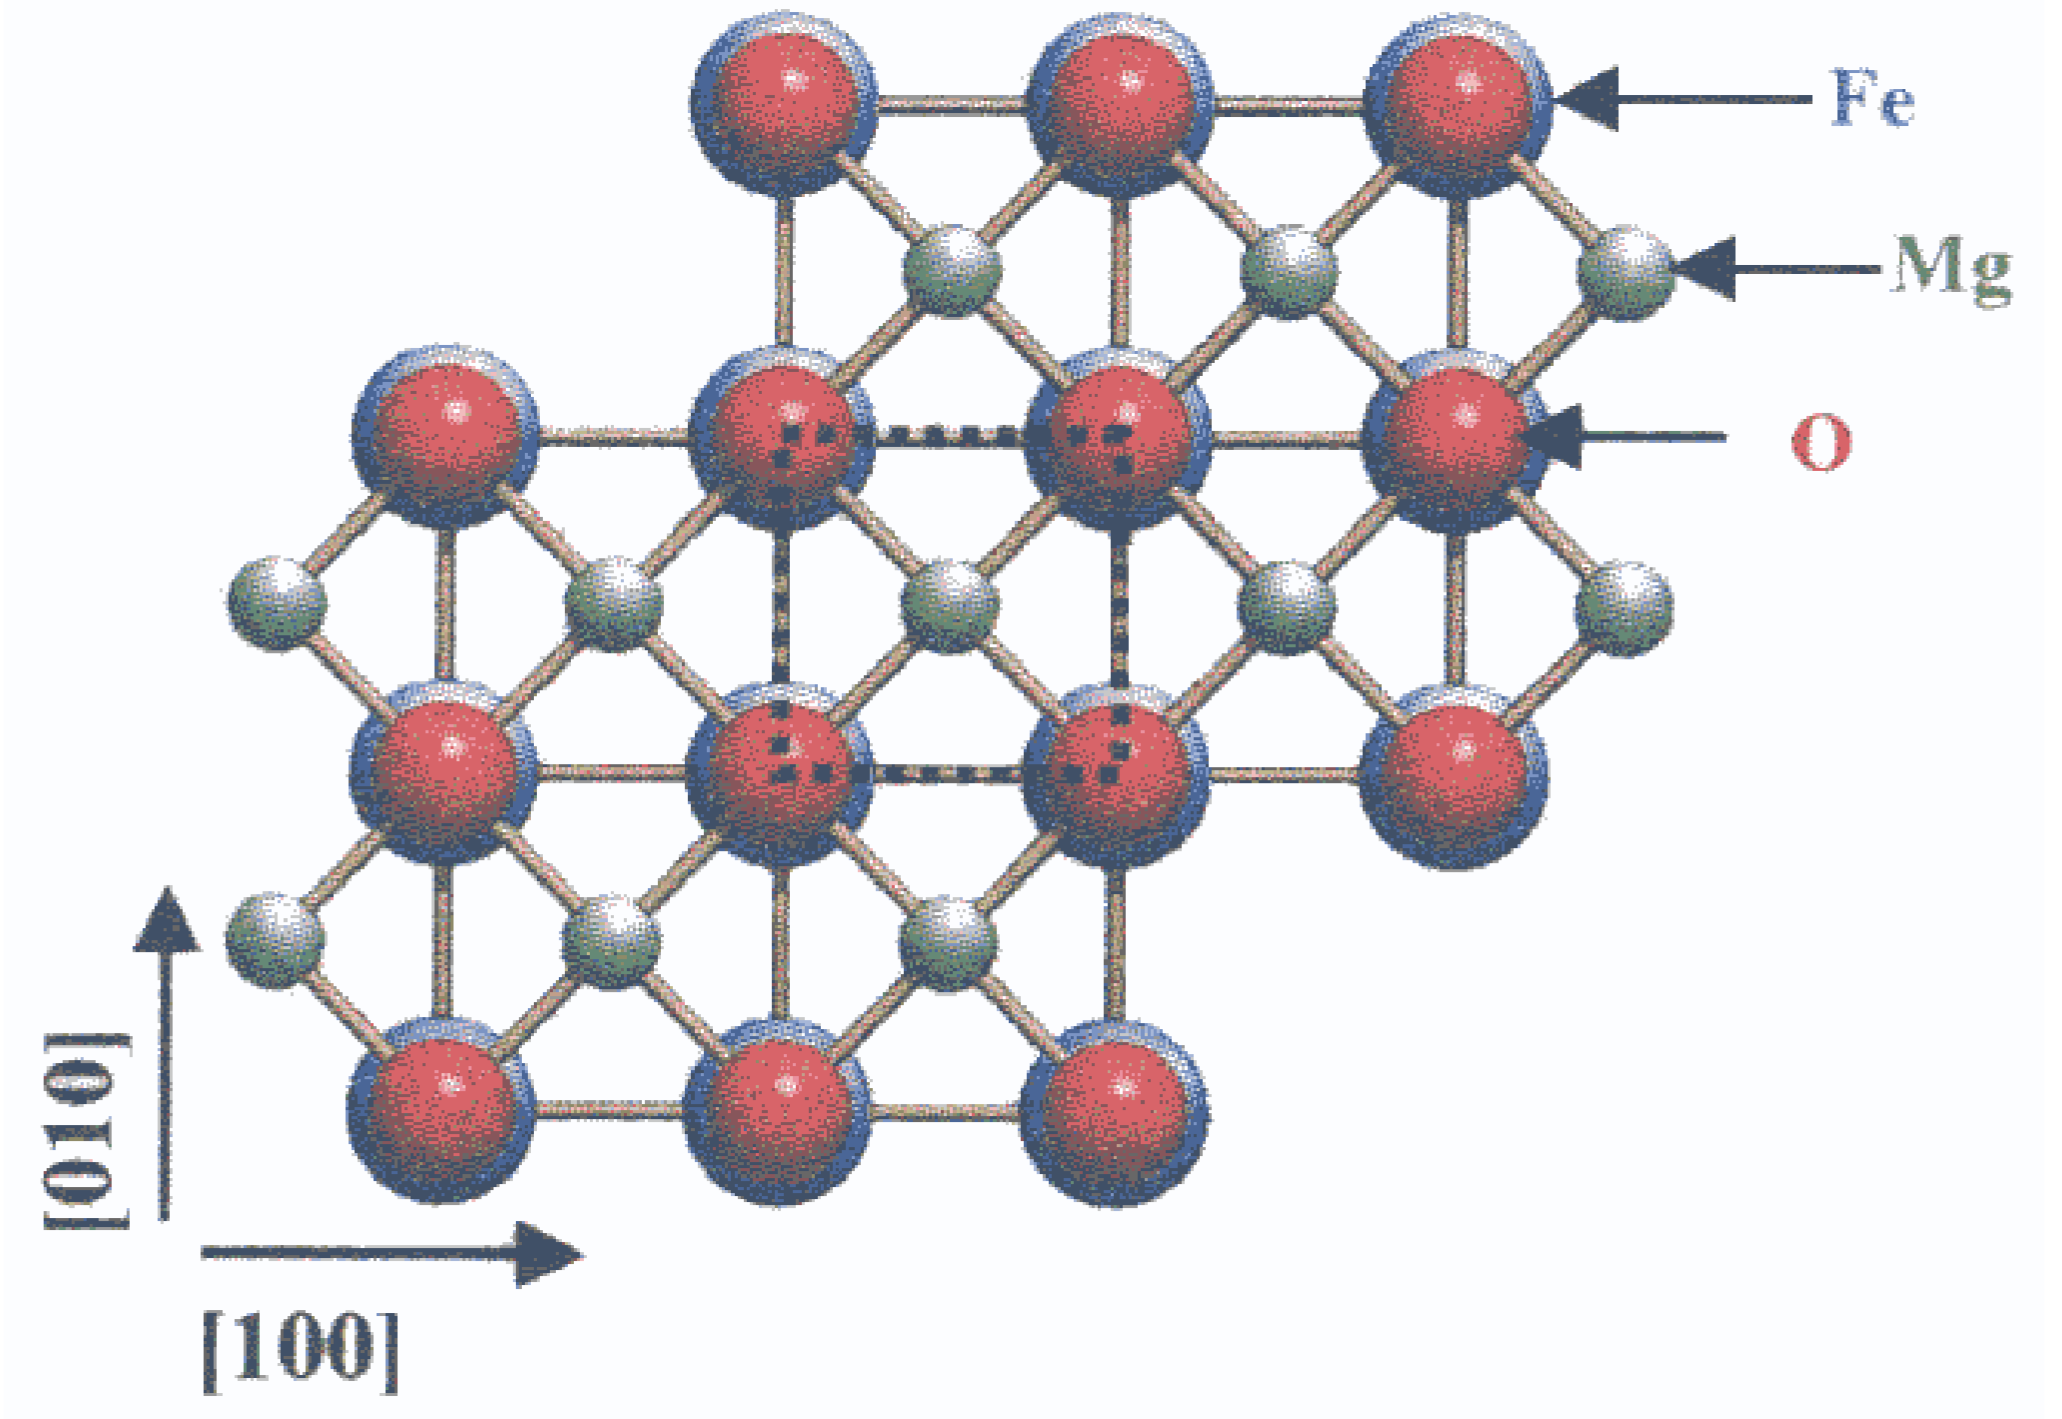
\includegraphics[width=0.45\linewidth]{Plots/Fe_MgO_Struktur.png}
    \caption{Anordnung einer Lage MgO auf Fe(100) in der Draufsicht. Die Sauerstoffionen liegen auf den Eisenatomen, während die Magnesiumionen 
    nach der NaCl-Struktur von MgO zwischen den Sauerstoffplätzen liegen.
    Die Richtungsangaben beziehen sich auf das Fe-System \cite{meyerheim2001geometrical}.}
    \label{fig:Fe_MgO}
\end{SCfigure}

Wenn sowohl Substrat als auch Adsorbat einkristallin sind 
und die wachsende Schicht eine wohldefinierte Beziehung zum Substrat hat, spricht man von Epitaxie.
Beim Wachstum von MgO auf Fe(100) und Fe(100)-p(1\,x\,1)O liegt die [100]-Richtung des Magnesiums in [110]-Richtung 
des Eisens, sodass die Sauerstoffionen auf den Eisenatomen liegen. Es entsteht eine Struktur wie schematisch in Abbildung \ref{fig:Fe_MgO} zu sehen, bei der 
die Gitterkonstante von MgO um $3,7\,\si{\percent}$ vom Atomabstand $\sqrt{2}\cdot 2,87\,\si{\angstrom}=4,06\,\si{\angstrom}$ von Eisen in [110]-Richtung abweicht. 
MgO kann bis zu einer Schichtdicke von 6 ML epitaktisch wachsen \cite{klaua2001growth}, erst danach bilden sich Versetzungen in Folge der 
Fehlanpassung der Gitterkonstanten \cite{dynna1996low}.

Beim Aufdampfen von Mg in einer Sauerstoffatmosphäre kann die Stöchiometrie direkt kontrolliert werden. 
Tekiel et al. \cite{tekiel2013reactive} fanden ein optimiertes Verhältnis der Mg-Aufdampfrate $r$ zum Sauerstoffdruck $p$ von 

\begin{equation}
    \dfrac{r}{p}=(0,15\pm 0,05)\cdot 10^8 \,\si{\angstrom\per\milli\bar\per\minute}.
    \label{eq:V1}
\end{equation}

Auf diese Weise können MgO-Filme mit hoher Stöchiometrie und kristalliner Struktur produziert werden.